\documentclass[a0paper,portrait]{baposter}

\usepackage[utf8]{inputenc}
\usepackage{relsize}	       % For \smaller
\usepackage{url}			       % For \url
\usepackage{multicol}        % Multi Columns
\renewcommand{\familydefault}{\sfdefault}
\usepackage{todonotes}

%%%%%%%%%%%%%%%%%%%%%%%%%%%%%%%%%%%%%%%%%%%%%%%%%%%%%%%%%%%%%%%%%%%%%%%%%%%%%%%%
%%% Utility functions %%%%%%%%%%%%%%%%%%%%%%%%%%%%%%%%%%%%%%%%%%%%%%%%%%%%%%%%%%
%%%%%%%%%%%%%%%%%%%%%%%%%%%%%%%%%%%%%%%%%%%%%%%%%%%%%%%%%%%%%%%%%%%%%%%%%%%%%%%%

%%% Save space in lists. Use this after the opening of the list %%%%%%%%%%%%%%%%
\renewcommand{\vec}[1]{\bm{#1}}
\newcommand{\vnabla}{\vec{\nabla}}

\renewcommand{\d}[1]{\text{d} #1}
\newcommand{\dxx}{\,\text{d}\vec{x}}
\newcommand{\dx}{\,\text{d}x}

\newcommand{\diff}[2]{\frac{\text{d}#1}{\text{d}#2}}
\newcommand{\idiff}[2]{\text{d}#1 / \text{d}#2}
\newcommand{\pdiff}[2]{\frac{\partial #1}{\partial #2}}
\newcommand{\pdifff}[2]{\frac{\partial^2 #1}{\partial #2^2}}
\newcommand{\ipdiff}[2]{\partial #1 / \partial #2}
\newcommand{\vdiff}[2]{\frac{\delta #1}{\delta #2}}
\newcommand{\ivdiff}[2]{\delta #1 / \delta #2}

%%%%%%%%%%%%%%%%%%%%%%%%%%%%%%%%%%%%%%%%%%%%%%%%%%%%%%%%%%%%%%%%%%%%%%%%%%%%%%%
%%% Document Start %%%%%%%%%%%%%%%%%%%%%%%%%%%%%%%%%%%%%%%%%%%%%%%%%%%%%%%%%%%%
%%%%%%%%%%%%%%%%%%%%%%%%%%%%%%%%%%%%%%%%%%%%%%%%%%%%%%%%%%%%%%%%%%%%%%%%%%%%%%%

\definecolor{HPCCFColor}{HTML}{181c57}


\begin{document}
\typeout{Poster rendering started}

%%% General Poster Settings %%%%%%%%%%%%%%%%%%%%%%%%%%%%%%%%%%%%%%%%%%%%%%%%%%%
%%%%%% Eye Catcher, Title, Authors and University Images %%%%%%%%%%%%%%%%%%%%%%
\begin{poster}{
  columns=3,
	grid=false,
	borderColor=HPCCFColor,
	headerColorOne=HPCCFColor,
	headerColorTwo=HPCCFColor,
	headerFontColor=white,
  headerheight=10em,
	boxColorOne=white,
  boxpadding=1em,
	headershape=rounded,
	headerfont=\Large\textsf,
	textborder=rounded,
	background=shadetb,
  bgColorOne=white,
  %bgColorTwo=white,
  bgColorTwo=blue!10,
	headerborder=open,
  boxshade=plain,
  eyecatcher=false
}
%%% Eye Cacther %%%%%%%%%%%%%%%%%%%%%%%%%%%%%%%%%%%%%%%%%%%%%%%%%%%%%%%%%%%%%%%
{
}
%%% Title %%%%%%%%%%%%%%%%%%%%%%%%%%%%%%%%%%%%%%%%%%%%%%%%%%%%%%%%%%%%%%%%%%%%%
{
\centering
\Huge \textcolor{HPCCFColor}{The International HPC Certification Program}}
%%% Authors %%%%%%%%%%%%%%%%%%%%%%%%%%%%%%%%%%%%%%%%%%%%%%%%%%%%%%%%%%%%%%%%%%%
{
  \centering
  \url{https://www.hpc-certification.org/}\\

  \vspace*{0.5em}

  Julian Kunkel$^1$, Kai Himstedt$^2$, Weronika Filinger$^3$, Jean-Thomas Acquaviva$^4$, William Jalby$^5$, Lev Lafayette$^6$, \\[-0em] Anja Gerbes$^7$, Waseem Kamleh$^8$, Sharan Kalwan$^9$

  \vspace*{-0.25em}

  {\scriptsize $^1$:University of Reading, $^2$:Universität Hamburg, $^3$:EPCC, $^4$:DDN, $^5$:Université de Versailles Saint-Quentin, $^6$:University of Melbourne, $^7$:University of Frankfurt, $^8$:University of Adelaide, $^9$:DataSwing}

  \vspace*{-0.5em}
}
%%% Logo %%%%%%%%%%%%%%%%%%%%%%%%%%%%%%%%%%%%%%%%%%%%%%%%%%%%%%%%%%%%%%%%%%%%%%
{%\begin{minipage}{20.0em}
    %\includegraphics[height=5em]{logo-uni}
 % \end{minipage}
}

%%% Abstract %%%%%%%%%%%%%%%%%%%%%%%%%%%%%%%%%%%%%%%%%%%%%%%%%%%%%%%%%%%%%%%%%%
\headerbox{Abstract}{name=abstract,column=0,row=0,span=2}{
\vspace*{-0.3em}
\begin{multicols}{2}
\textit{%
The HPC community has always considered the training of new and existing HPC practitioners to be of high importance to its growth. The significance of training will increase even further in the era of Exascale when HPC encompasses even more scientific disciplines. This diversification of HPC practitioners challenges the traditional training approaches, which are not able to satisfy the specific needs of users, often coming from non-traditionally HPC disciplines and only interested in learning a particular set of skills. HPC centres are struggling to identify and overcome the gaps in users’ knowledge. How should we support prospective and existing users who are not aware of their own knowledge gaps?
}

\medskip

\textit{%
We started the establishment of the International HPC Certification program that aims to clearly categorize, define and examine HPC related skills.
Oriented on the needs of practitioners, the program does not define a linear curriculum or interfere with content providers.
Ultimately, we aim for the certificates to be recognized and respected by the HPC community and industry.
}
\end{multicols}
}


\headerbox{Competences and Skills}{name=box12,column=0,below=abstract, span=2}{
Various competencies are necessary to efficiently use HPC resources.
A skill is a meaningful competence that comes with a \textbf{clear definition} of knowledge/practical ability, \textbf{levels of knowledge}, \textbf{relations to other skills}.
An excerpt of the first levels of the skill-tree:

\medskip

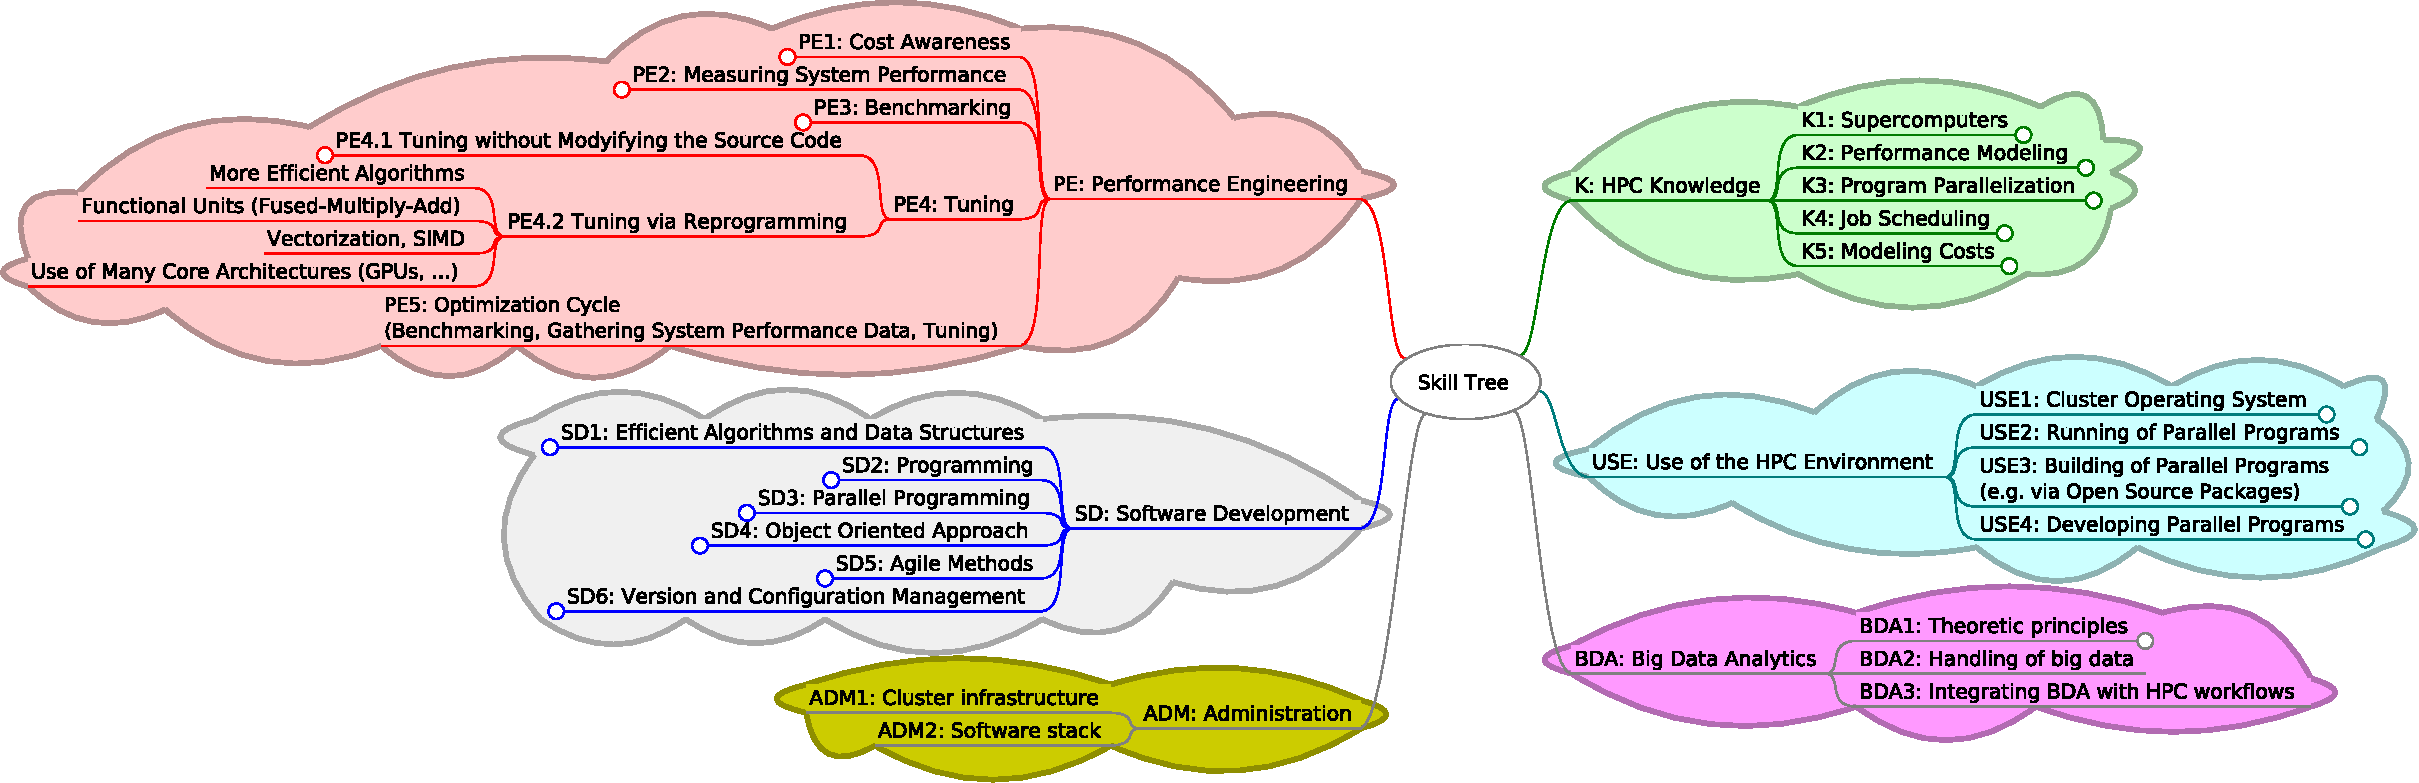
\includegraphics[width=1\textwidth]{1-crop.pdf}
%\includegraphics[width=\textwidth, height=6cm]{skill-tree-auto-generated_180412a.png}
% \includegraphics[width=\textwidth, trim=2cm 28cm 2cm 0cm, clip]{skill-tree-auto-generated_180412a.pdf}

\medskip


The skill-handbook is available in various representations on the webpage and on our GitHub.
}

\headerbox{Benefits}{name=benefits,column=0,below=box12}{
  %\begin{columns}
   % \column{0.5\textwidth}
    \textbf{HPC practitioners}
    \vspace*{-0.5em}
      \begin{itemize}
        \setlength\itemsep{-0.3em}
      \item Increase motivation to participate
      \item (Certificates are recognized in CV)
      \item Validate knowledge via tests
      \item Browse of relevant competences
      \item Identify recommended and required skills
      \item Compare teaching offers across sites
  	  \end{itemize}

	%\column{0.5\textwidth}
    \textbf{Data centers}
    \vspace*{-0.5em}
      \begin{itemize}
        \setlength\itemsep{-0.3em}

      \item Increase sharing of teaching materials
      \item Documentation of taught skills simplified
      \item Identify missing teaching activities
      \item Tailor skill-tree specifically to users
      \item Correlate lack of skills with efficient use
  	  \end{itemize}
  %\end{columns}%
}

\headerbox{Example Skill (Excerpt)}{name=status,column=0,below=benefits, above=bottom}{

\textbf{ID}: USE4.2.1-B \\
\textbf{Name}: Workload manager introduction \\
\textbf{Background} \\
\textit{\scriptsize There is a wide range of different workload managers in use. This skill covers generic and widely used concepts.}

\textbf{Objectives} \\
\textit{\scriptsize
comprehend and describe the basic architecture and concepts of resource allocation for an HPC system
}

\textbf{Outcomes} \\
\textit{\scriptsize
  - comprehend the exclusive and shared usage model in HPC \\
  - differentiate batch and interactive job submission \\
  - comprehend the generic concepts and architecture of ... \\
  - explain environment variables as a means to communicate \\
  - explain the generic steps to run and monitor a single job
}
}


\headerbox{Get Involved!}{name=box2,column=1,below=box12,above=bottom}{
This is an independent community-wide effort.

\bigskip

\textbf{Who can join?}

%\begin{itemize}
%\item
Anyone (person or organization) experienced or interested in HPC teaching and training.
%\end{itemize}

\bigskip

\textbf{What can we contribute?}

There are various levels of contribution
\vspace*{-0.4em}
\begin{itemize}
\setlength\itemsep{-0.3em}
\item developing skill-tree scope and content
\item becoming ambassador for the program
\item steering of the governance body
\end{itemize}
\vspace*{-0.4em}

Simply visit our website \url{hpc-certification.org} and join the mailing lists!

\bigskip

\textbf{What does it cost to join?}

It is free to join for everyone!
However, for \textbf{full members} (with voting rights), we expect a minimum contribution to the overall program.
Note that anyone joining will be listed on the public webpage!

\medskip
\textbf{Meetings:}

A general assembly of members will occur at least twice a year -- during ISC and SC.
On a monthly basis, the program chair organizes a conference call, that shall be attended by the executive board but is open to members.

\medskip
\textbf{Providing teaching material:}

Since the certification program itself curates the curriculum but does not provide teaching material, anyone is welcome to provide teaching material -- we support branding of the material!
}

\headerbox{The PeCoH Project}{name=pecoh,column=2}{
	The Performance Conscious HPC (PeCoH) project* aimed to create a lightweight HPC certification program. During the first year, it became apparent to broaden the scope and form an independent governance entity to sustain the effort and gain acceptance. Project information:
    \begin{itemize}%[noitemsep,nolistsep]
    \item DFG funded (runtime: 2017-2019)
    \item Partners
    	\vspace*{-0.5em}
    	\begin{itemize}
        \item Universität Hamburg (UHAM)
        \item Regional computing center UHAM
        \item Computer Center of Hamburg University of Technology (TUHH RZ)
        \end{itemize}
    \item Methods:
    	\vspace*{-0.5em}
    	\begin{itemize}
        	\item Competence management
            \item Cost-Awareness
            \item Success stories
            \item Explore benefit of new concepts
		\end{itemize}
    \end{itemize}
	{\tiny *:\url{https://wr.informatik.uni-hamburg.de/research/projects/pecoh/} }
}




\headerbox{Status}{name=next,column=2,below=pecoh}{

PeCoH contributed a concept paper, skill-tree, and a Javascript visualization to the effort.

Technically, skills are stored in an XML document and can be processed via XSLT into various representations; they are also available as Markdown.

The Javascripts can be re-used and configured by anyone -- e.g., for linking teaching material.

We established a set of rules with the members of the forum and voted for the members of the steering board.


\smallskip

\textbf{Responsibilities of the governance body}:
\vspace*{-0.5em}
  \begin{itemize}
  \setlength\itemsep{-0.3em}
  \item Steering the program
  \item Curating the curriculum
  	%\vspace*{-0.5em}
  	%\begin{itemize}
%    	\setlength\itemsep{0em}
 %   	\item Curating the skill-handbook
  %      \item Defining certificates on skill sets
   % \end{itemize}
  \item Performing the exams
  	%\vspace*{-0.5em}
  	%\begin{itemize}
    %\setlength\itemsep{0em}
    %\item First approach: Online
    %\end{itemize}
  \end{itemize}
  \vspace*{-0.5em}
It is \textbf{not} its duty to interfere with content! We aim to preserve the teaching ecosystem.

\smallskip

\textbf{Next steps}

\hrule

\medskip

We are completing the definition of the skills including the learning outcomes and extending the skill tree with administrative and big-data relevant skills.

%A first meeting takes place during ISC-HPC to establish initial governance rules, and define next steps. Everyone is welcome to attend.
%\textbf{When}: Wed. 27. Jun. 2018 12:45 – 13:30 (bring your lunch) \\
%\textbf{Where}: Exhibition hall, Lunch area, table closest to booth N-230 (project posters)


%The meeting takes place on \textbf{TODO fill final slot here}.
}

\headerbox{Acknowledgements}{name=box32,column=2,below=next,above=bottom}{
\scriptsize
The PeCoH project is supported by the German Research Foundation (DFG) under grants LU 1353/12-1, OL 241/2-1, and RI 1068/7-1.

\todo[inline]{Maybe add logos here}
}

\end{poster}
\end{document}
